En esta sección se entrará a describir con total detalle el contenido técnico de la aplicación. Partiendo desde un analisis de requisitos funcionales
hasta no funcionales, pasando por las tecnologías usadas para la implemetación de estos. 

\section{Tecnologias Empleadas}

\subsection{SpringBoot}
Spring Boot es un marco de trabajo Java que simplifica el desarrollo de aplicaciones web al eliminar la 
complejidad de la configuración manual. Ofrece configuración automática, empaquetado de aplicaciones independientes y un inicio rápido integrado, 
lo que permite a los desarrolladores crear aplicaciones de manera más rápida y eficiente, centrándose en la lógica de negocio en lugar de la configuración. 
Genial para el desarrollo de aplicaciones \textit{CRUD}\footnote{\textit{CRUD} es un acrónimo en inglés que se refiere a las operaciones 
básicas de manipulación de datos en aplicaciones informáticas: Create (Crear), Read (Leer), Update (Actualizar) y Delete (Eliminar).}.
\subsection{Maven}
Maven es una herramienta de gestión de proyectos Java que simplifica la estructuración, gestión de dependencias y automatización de la construcción. 
Permite definir dependencias en un archivo de configuración (pom.xml), ejecutar fases de construcción estandarizadas y gestionar repositorios 
centralizados de bibliotecas. Es ampliamente utilizado en el desarrollo Java por su integración con IDEs y su capacidad para proyectos multiproyecto, es decir,
permite la gestión de múltiples proyectos en un solo repositorio, lo que facilita la colaboración entre desarrolladores y la gestión.
\subsection{Vue.js}
Vue.js es un popular marco de trabajo de código abierto para construir interfaces de usuario interactivas en aplicaciones web de una sola página. 
Se destaca por su enfoque centrado en el componente, su sintaxis declarativa y su eficiente sistema de reactividad. Vue.js facilita la construcción 
de aplicaciones web complejas al fomentar la reutilización de componentes y ofrecer herramientas integradas para la manipulación del DOM y la gestión 
del estado de la aplicación.

\subsection{MySQL}
MySQL es un sistema de gestión de bases de datos relacional de código abierto ampliamente utilizado en el desarrollo de 
aplicaciones web y empresariales. Destaca por su escalabilidad, rendimiento, fiabilidad y facilidad de uso. Ofrece opciones 
sólidas de seguridad y es compatible con una variedad de plataformas y lenguajes de programación. MySQL es una herramienta poderosa 
para gestionar eficientemente grandes volúmenes de datos y garantizar la integridad y disponibilidad de la información.

\subsection{IntelliJ}
IntelliJ IDEA es un entorno de desarrollo integrado (IDE) altamente productivo desarrollado por JetBrains. 
Diseñado para diversas tecnologías, ofrece una interfaz de usuario intuitiva y funciones avanzadas que mejoran la 
productividad del desarrollador. Con soporte para múltiples lenguajes y marcos de trabajo, integración con herramientas de desarrollo y 
características colaborativas, IntelliJ IDEA es una opción popular para el desarrollo de software en Java y otros lenguajes.

\subsection{VSCode}
Visual Studio Code (VSCode) es un IDE popular desarrollado por Microsoft, conocido por su versatilidad, rendimiento y comunidad activa.
 Ofrece características avanzadas y extensiones para diferentes lenguajes de programación. Es altamente personalizable y cuenta con una 
 amplia documentación disponible en su sitio web oficial.

\subsection{AWS S3}
AWS S3 es un servicio de almacenamiento en la nube ofrecido por Amazon Web Services. Destaca por su escalabilidad, durabilidad, seguridad y 
facilidad de uso. Permite almacenar grandes cantidades de datos de forma segura y acceder a ellos de manera eficiente a través de una interfaz 
intuitiva y una API robusta. Con una estructura de precios flexible, AWS S3 es una opción atractiva para empresas que buscan una solución de 
almacenamiento en la nube rentable y confiable.

\subsection{AWS EC2}
AWS EC2 es un servicio de cómputo en la nube proporcionado por Amazon Web Services. Destaca por su escalabilidad, flexibilidad y seguridad. 
Permite a los usuarios alquilar capacidad informática según sus necesidades, con opciones de pago por uso. Es fácil de usar y ofrece una variedad 
de opciones de implementación. En resumen, EC2 es una solución eficiente y confiable para ejecutar aplicaciones y cargas de trabajo en la nube.

\subsection{Docker}
Docker es una plataforma de código abierto que permite crear, implementar y ejecutar aplicaciones en contenedores. Destaca por su portabilidad, 
eficiencia y facilidad de uso. Con la tecnología de contenedores, Docker ofrece aislamiento de aplicaciones y escalabilidad, lo que simplifica el 
desarrollo y la administración de aplicaciones en diferentes entornos. En resumen, Docker es una herramienta fundamental para la creación y gestión 
eficiente de aplicaciones modernas.

\newpage
\section{Resumen de las tecnologias}
La Tabla \ref{tabla:tecnologias_usos} recoge un resumen de las tecnologías empleadas para el desarrollo de Enterprise Event Solutions
\begin{table}[h]
\begin{tabular}{ p{3cm} l  }

    \hline
    Tecnologia& Uso \\
    \hline
    SpringBoot   & Framework \\
    Maven &   Framework \\
    Vue.js & Framework  \\
    MySQL    & Tecnologia de BD \\
    IntelliJ&   Entorno de Desarrollo  \\
    VSCode& Entorno de Desarrollo \\
    AWS S3& Tecnologia de de BD en la nube  \\
    AWS EC2& Servidor web en la nube  \\
    Docker& Crecion de imagenes comprimidas para despliegue  \\
    \hline
   \end{tabular}
   \caption{Tecnologías y sus usos correspondientes}
   \label{tabla:tecnologias_usos}
\end{table}
\newpage
\section{Arquitectura}
\textbf{Enterprise Event Solutions} es una aplicación \textbf{Fullstack} creada siguiendo un patrón de diseño MVC. A continuación, se muestra un plano general
que será desglosado:  CAMBIAR DIAGRAMA !!!!1 AÑADIR SEGURIDAD 

\section*{Arquitectura General}
\begin{figure}[h]
    \centering
    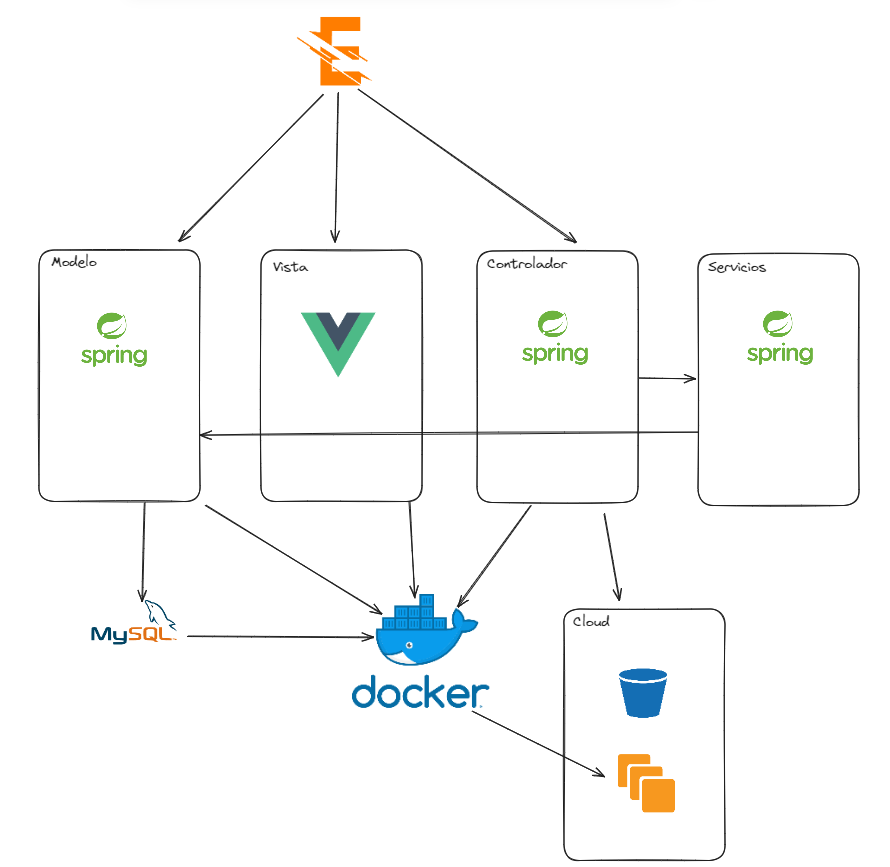
\includegraphics[width=0.8\textwidth]{Arquitectura.png} 
    \caption{Diagrama de Arquitectura de EVS}
    \label{fig:mvc_architecture}
\end{figure}
\newpage

\section*{Backend (Modelo y Controlador)}

\begin{itemize}
    \item \textbf{Tecnología}: \textbf{SpringBoot}
    \item \textbf{Descripción}: Utilizado por su gran versatilidad para manejar la lógica de negocio y control de la aplicación. Gracias a esto, el frontend
    de la aplicación se sirve directamente desde el Servidor de Apache proporcionado por spring, es decir, tengo empaquetado el tanto el back como el front en la misma ip
    y en el mismo puerto.
\end{itemize}

\section*{Frontend (Vista)}

\begin{itemize}
    \item \textbf{Tecnología}: \textbf{Vue.js}
    \item \textbf{Descripción}: Seleccionado para explorar otras tecnologías y facilitar la creación de una interfaz de usuario interactiva.
\end{itemize}

\section*{Tecnologías Complementarias}

\begin{itemize}
    \item \textbf{AWS EC2}: 
    \begin{itemize}
        \item \textbf{Descripción}: Instancia EC2 para desplegar la aplicación, ofreciendo un entorno robusto y escalable.
    \end{itemize}
    \item \textbf{AWS S3}:
    \begin{itemize}
        \item \textbf{Descripción}: Bucket S3 para almacenar imágenes, reduciendo la carga de trabajo en la base de datos.
    \end{itemize}
    \item \textbf{MySQL}:
    \begin{itemize}
        \item \textbf{Descripción}: Base de datos utilizada para gestionar los datos de la aplicación de manera eficiente.
    \end{itemize}
\end{itemize}

\textbf{Enterprise Event Solutions} combina las fortalezas de \textbf{SpringBoot} y \textbf{Vue.js} en un patrón MVC para ofrecer una solución robusta y 
escalable. Con el soporte de \textbf{AWS} y \textbf{MySQL}, la aplicación está preparada para manejar grandes volúmenes de datos y ofrecer una experiencia 
de usuario fluida.


Cada uno de los componentes definidos en la Imagen \ref{fig:mvc_architecture} será desglosado en las próximas secciones para explicar detalladamente el contenido de 
la aplicación.

\subsection{Modelo}
La persistencia en Enterprise Event Solutions se sustenta en una serie de Entidades almacenadas en una base de datos con la que los servicios interactuan mediante
las interfaces proporcionadas por JPA \ref{sec:jpa}. Es el pilar fundamental en el que se sustenta el modelo de negocio de la aplicación.
\begin{figure}[h]
    \centering
    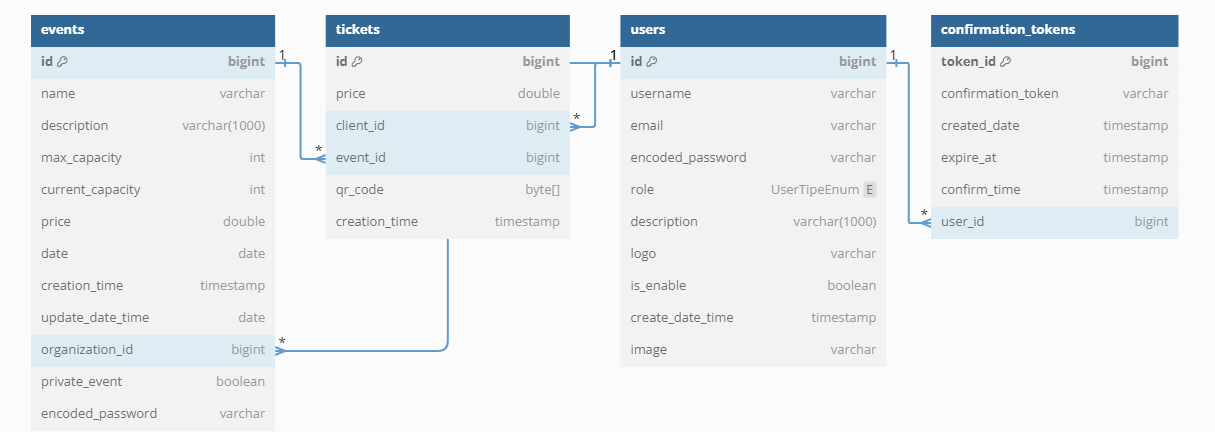
\includegraphics[width=1.2\textwidth]{EVSdiagra.png} 
    \caption{Modelo E-R de la BD}
    \label{fig:diagramaBD}
\end{figure}

\subsubsection{JPA}
\label{sec:jpa}

JPA (Java Persistence API) es una especificación de Java que facilita la gestión de la persistencia de datos en aplicaciones Java.
En Spring, se usa para simplificar las operaciones CRUD y el manejo de relaciones entre entidades, permitiendo trabajar con objetos en lugar de SQL. 
Spring Data JPA integra JPA en el ecosistema Spring, proporcionando repositorios predefinidos para operaciones de base de datos comunes.

A continuación se muestra un fragmento de código de Spring Data JPA en Java:
\myjavastyle
\begin{lstlisting}[language=Java, caption=Ejemplo de Repositorio en Spring Data JPA]
@Repository
public interface UserRepository extends JpaRepository<User,Long> {
    public Optional<User> findByEmail(String email);
    public List<User> findAllByRole(UserTipeEnum type);
    public Optional<User> findByUsername(String username);
}
\end{lstlisting}

Como se puede observar, gracias a la gran potencia de Spring y de JPA, simplemente con crear una interfaz con metodos que creemos que vamos a necesitar en 
nuestros servicios, y sin la necesidad de añadir @Querys, podemos hacer consultas sobre la base de datos.

Pero también podemos hacer nuestras propias Querys sobre la base de datos:
\myjavastyle
\begin{lstlisting}[language=Java, caption=Ejemplo de Query  en Spring Data JPA]
    @Transactional
    @Modifying
    @Query("UPDATE Event e SET e.current_capacity = e.current_capacity + 1 WHERE e.id = :id AND e.current_capacity + 1  <= e.max_capacity")
    public int incrementCurrentCapacity(@Param("id") Long id);
\end{lstlisting}

\subsection{Contolador}
La creación de controladores me ha permitido gestionar un sistema de endpoints que sirve como la interfaz principal 
para la comunicación entre el cliente y el servidor. Estos controladores se encargan de recibir las solicitudes HTTPS de delegar el procesamiento a 
los servicios correspondientes. Los servicios encapsulan la lógica de negocio y se comunican con los repositorios JPA para acceder a los datos de la 
base de datos de manera eficiente. Además, para garantizar la seguridad, se utiliza JWT (JSON Web Tokens), que permite la autenticación y autorización 
de los usuarios. Los tokens JWT se generan tras un inicio de sesión exitoso y se utilizan para proteger los endpoints, asegurando que solo los usuarios 
autenticados puedan acceder a recursos específicos. Este enfoque no solo organiza el código de manera modular y mantenible, sino que también proporciona 
una robusta capa de seguridad para la API.
\begin{figure}[h]
    \centering
    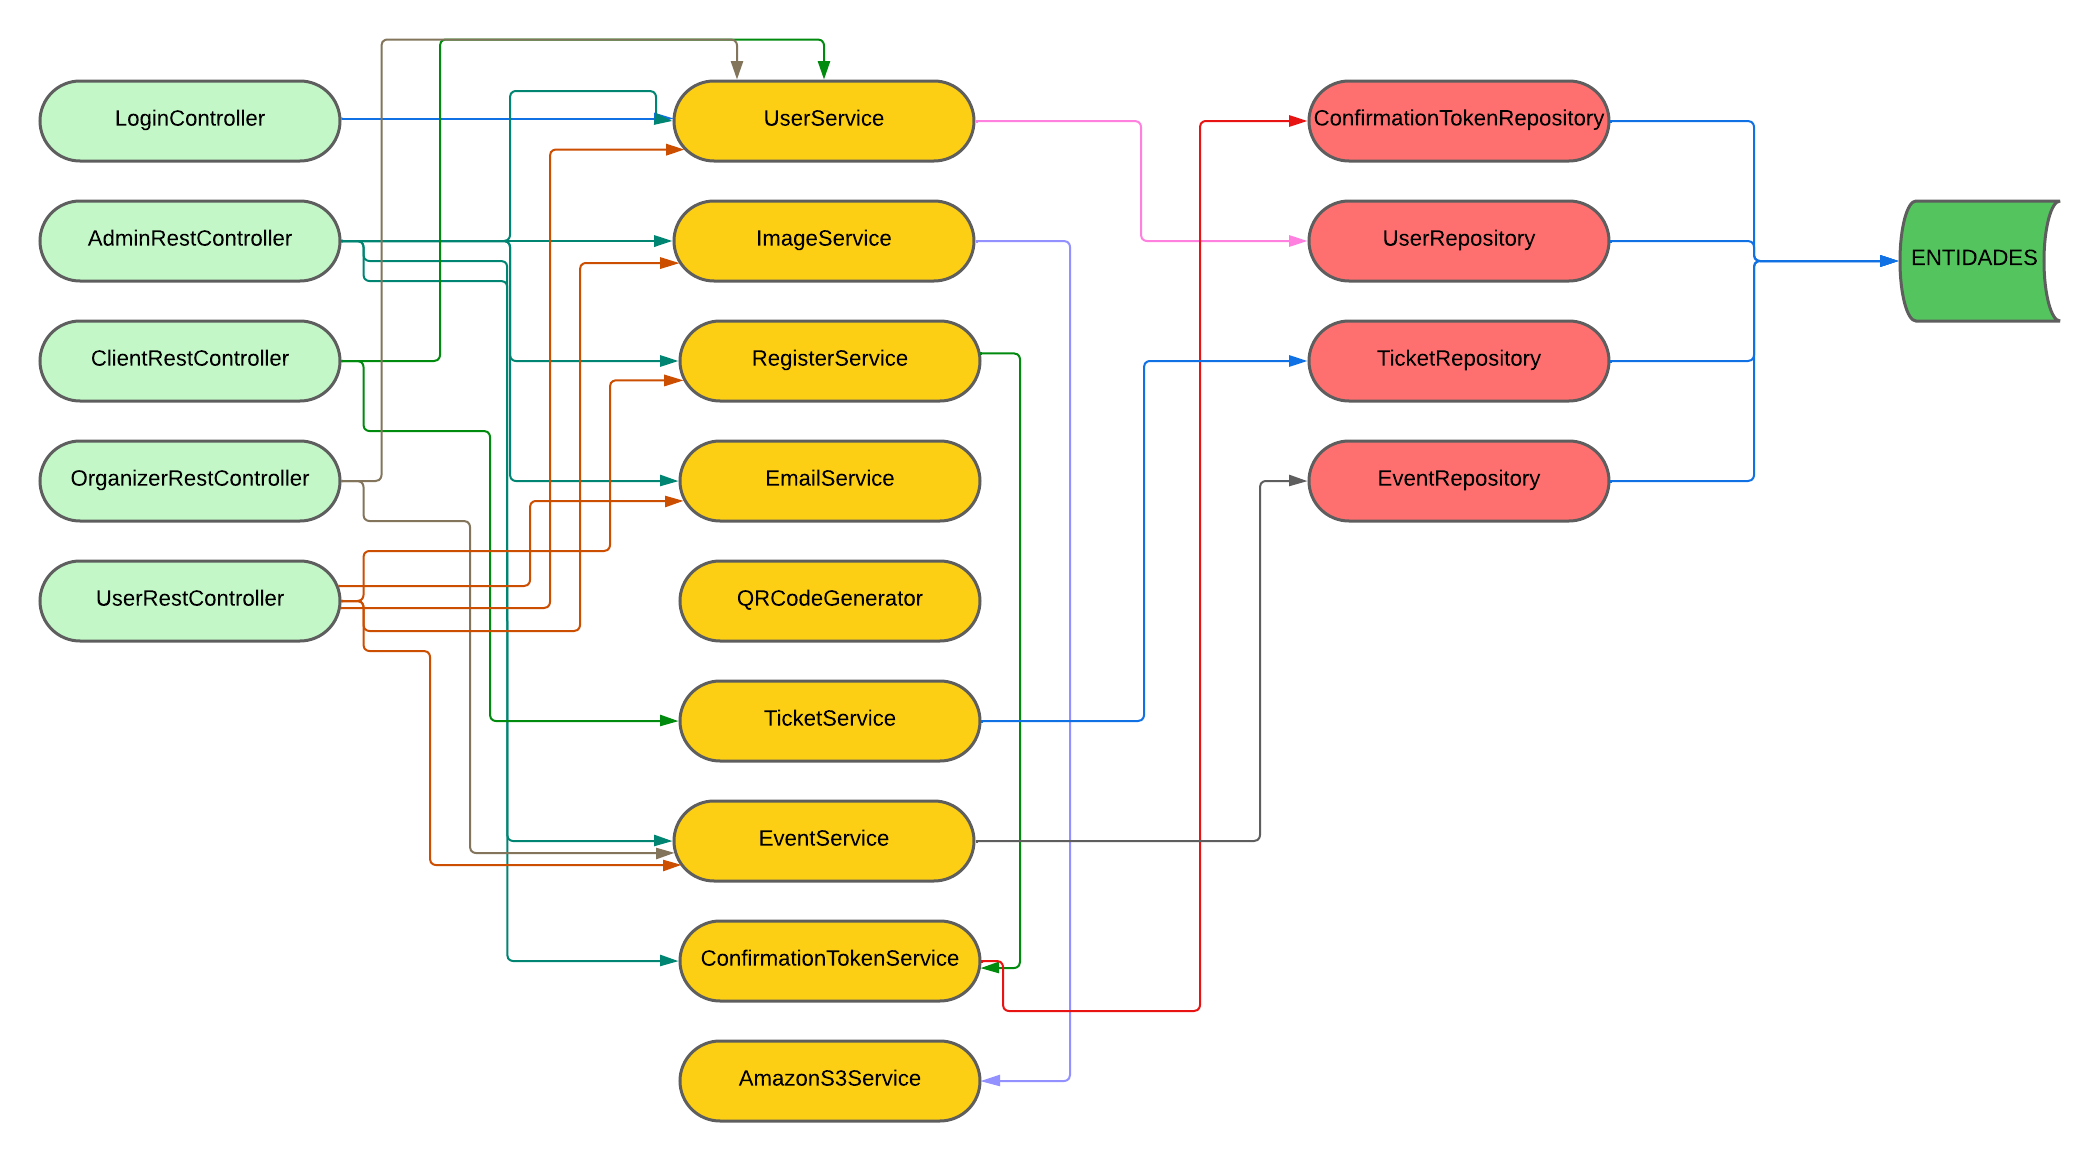
\includegraphics[width=1\textwidth]{DiagramaClases.png} 
    \caption{Diagrama de Clases de EVS}
    \label{fig:class_architecture}
\end{figure}

Además he implementado otras configuraciones para añadir una capa extra de seguridad a la aplicación como configuración CSRFH y Cors para limitar las url 
que pueden hacer uso de los endpoints de mi app. Por supuesto he creado las configuraciones necesarias para manejar las tecnologias externas como S3, dentro de 
EVS.
\begin{figure}[h]
    \centering
    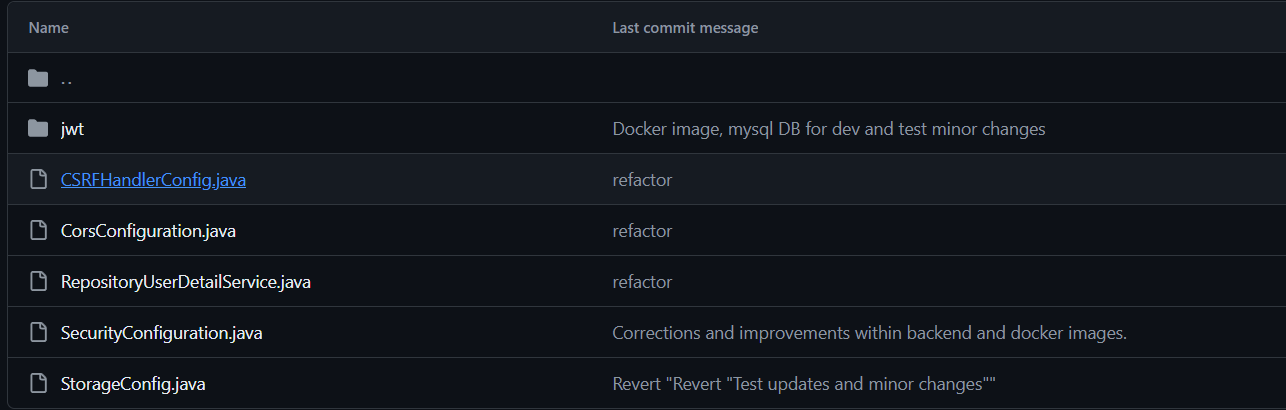
\includegraphics[width=1\textwidth]{security.png} 
    \caption{Seguridad del backend}
    \label{fig:securityClasses}
\end{figure}

\subsection{Vista}
El frontend de Enterprise Event Solution ha sido implementado en Vue.js. Especificamente en Vue3, que trae consigo algunos cambios con respecto a su versión
anterior Vue2. La utilización de este framework me ha permitido añadir tanto bibliotecas de componentes y gráficos (Bootstrap5 y Chart.js respectivamente)
como relaciones entre los diferentes componentes basado en "props", permitiendo de esta manera diferentes comportamientos del componente dependiendo de
que valores se le pasen en el componente padre.

Un ejemplo del uso de estas props sería:
\myvuestyle
\begin{lstlisting}[language=HTML, caption=Ejemplo del Padre, label=lst:padre]
    <event_cards
    :evento="evento"
    :is-org="false"
    >
    </event_cards>
\end{lstlisting}
\myvuestyle
\begin{lstlisting}[language=HTML, caption=Ejemplo del Hijo, label=lst:hijo]
    <script lang="ts">
    import {EventService} from "../services/event.service";
    import { useRouter } from "vue-router";
    import { Event } from "../models/Event";
    import { computed, ref } from "vue";
    export  default {
        name: "event_cards",
        props:{
          evento: Object as ()=> Event,
          isOrg: Boolean,
        },
    }
\end{lstlisting}

En el código \ref{lst:padre}, se observa que se inserta en el template un componente con la información del evento. Por otro lado, en el código 
\ref{lst:hijo}, se manejan estos valores que hemos pasado desde el componente padre. En este fragmento, si se le pasa \texttt{true} en la variable 
\texttt{is-org}, el componente tendrá un comportamiento diferente a si se le pasa \texttt{false}. Ademas en la variable \texttt{evento} le pasamos la información
del evento para garantizar la reactividad de los componetes de forma individual. De esta forma trabajamos con módulos y no con un elemento.

\newpage
A continuación se muestra un diagrama con las Pantallas de la aplicación y sus acceso en función del tipo de usuario.
\begin{figure}[h]
    \centering
    \rotatebox{90}{
        \includegraphics[width=1\textwidth]{DiagramaFlujo.png}
    }
    \caption{Interfaz con el usuario}
    \label{fig:userInterface}
\end{figure}

\newpage
\subsection{Cloud}
Para mejorar la eficiencia y escalabilidad de la aplicación, he utilizado Amazon S3 para almacenar imágenes y reducir la carga en la base de datos, y 
Amazon EC2 para desplegar la aplicación, garantizando así un rendimiento óptimo y una alta disponibilidad. 

Uno de los objetivos a cumplir era el Despliegue Continuo,es decir, cada vez que realizara un cambio sobre la aplicación se automatizara el proceso 
de despliegue en la maquina EC2. 

En un primer momento la idea era crear un \texttt{workflow} de Github para automatizar esta tarea pero debido a la poca potencia de la maquina fisica de Amazon, 
en su versión gratuita, no fué posible ya que la RAM de este hardware alcanzaba el máximo de su capacidad simplemente al ejecutar el Runner configurado en el 
repositorio de Github.

Por ello, opté por crear un script para que simplemente desde la consola de la EC2 pudiera hacer este proceso de la forma más rápida posible.

\section{Especificación de Requisitos}
En esta sección se establecen las necesidades y expectativas a cumplir, así como los elementos clave que guían el diseño y la implementación de la aplicación.
\newpage
\subsection{Requisitos Funcionales}
La Tabla \ref{tabla:RF} recoge las funcionalidades específicas que el sistema debe ofrecer.

\begin{longtable}{ p{2.5cm} p{4cm} p{9cm}  }
    \caption{Requisitos Funcionales} \label{tabla:RF} \\
    \hline
    ID& Resumen& Descripción \\
    \hline
    \endfirsthead
    
    \multicolumn{3}{c}%
    {{\bfseries \tablename\ \thetable{}: Continuación de la tabla anterior}} \\
    \hline
    ID& Resumen& Descripción \\
    \hline
    \endhead
    
    \hline \multicolumn{3}{|r|}{{Continúa en la siguiente página}} \\ \hline
    \endfoot
    
    \hline
    \endlastfoot
    
    \textbf{RF-001}& Login y Registro & El sistema permitirá a los usuarios iniciar sesión con credenciales válidas o registrarse como nuevos 
    usuarios, proporcionando la funcionalidad básica de autenticación y creación de cuentas.\\
    \textbf{RF-002} & Edición completa del perfil por parte de los usuarios & Los usuarios dispondrán de la capacidad total para editar y
    actualizar la información de su perfil dentro del sistema, lo que incluirá datos personales y otros detalles relevantes, ofreciendo una 
    experiencia de usuario personalizada y adaptable.\\
    \textbf{RF-003} & Autorización de correo electrónico & Cuando un usuario se registre, se enviará un correo electrónico de verificación para 
    asegurar la autenticidad de la dirección de correo electrónico proporcionada.\\
    \textbf{RF-101} & Visualización de cantidad de usuarios registrados por mes & El administrador podrá ver la cantidad de usuarios que se han 
    registrado en el sistema durante cada mes.\\
    \textbf{RF-102} & Visualización de cantidad de usuarios por tipo & El administrador podrá ver la cantidad de usuarios registrados clasificados 
    por tipo (administrador, organizador, cliente) en el sistema.\\
    \textbf{RF-103} & Visualización de cantidad de eventos creados por mes & El administrador podrá ver la cantidad de eventos que se han creado en 
    el sistema durante cada mes.\\
    \textbf{RF-104} & Creación de usuarios de tipo Organización & Se dotará al administrador de la capacidad de crear usuarios con el rol específico 
    de 'Organización', lo que permitirá una gestión más detallada y especializada de usuarios dentro del sistema.\\
    \textbf{RF-105} & Filtrado de usuarios por tipo, nombre o email & Se integrará una función que permita al administrador obtener un 
    listado completo de todos los usuarios del sistema, con la posibilidad de aplicar filtros según su tipo de usuario, nombre o dirección 
    de correo electrónico para una búsqueda más eficiente y precisa.\\
    \textbf{RF-106} & Borrado de usuarios por parte del administrador & Se implementará la funcionalidad para que el administrador pueda 
    eliminar usuarios del sistema previa confirmación, permitiendo una gestión eficiente de la base de datos de usuarios y garantizando la integridad 
    y seguridad del sistema.\\
    \textbf{RF-107} & Obtener Usuario en el Sistema & Se implementará la funcionalidad para que el administrador pueda 
    ver información básicas de los usuarios registrados en el sistema\\
    \textbf{RF-201} & Ver eventos creados por el organizador & El organizador tendrá la capacidad de ver los eventos que ha creado dentro del sistema.\\
    \textbf{RF-202} & Eliminación de eventos por el organizador & Se permitirá al organizador eliminar los eventos que ha creado dentro del sistema.\\
    \textbf{RF-203} & Edición de eventos por el organizador & El organizador podrá editar los eventos que ha creado, lo que incluirá la modificación de 
    detalles como nombre, descripción, fecha, etc.\\
    \textbf{RF-204} & Creación de eventos por el organizador & Se permitirá al organizador crear nuevos eventos proporcionando detalles como nombre, descripción, 
    fecha y, opcionalmente, contraseña para acceder al evento.\\
    \textbf{RF-205} & Visualización de cantidad de inscritos en eventos por el organizador & El organizador podrá ver la cantidad de usuarios inscritos en los 
    eventos que ha creado dentro del sistema.\\
    \textbf{RF-301} & Visualización de organizaciones por parte del cliente & Los clientes tendrán la capacidad de ver las organizaciones disponibles en el sistema.\\
    \textbf{RF-302} & Visualización de perfil de organizaciones por parte del cliente & Los clientes podrán ver el perfil de las organizaciones dentro del sistema.\\
    \textbf{RF-303} & Visualización de eventos de organizaciones por parte del cliente & Los clientes podrán ver los eventos que ofrecen las organizaciones dentro del sistema.\\
    \textbf{RF-304} & Inscripción a eventos por parte del cliente & Los clientes podrán inscribirse a los eventos ofrecidos por las organizaciones dentro del sistema.\\
    \textbf{RF-305} & Eventos privados con contraseña & Se permitirá la creación de eventos privados que requieran una contraseña para acceder a ellos.\\
    \textbf{RF-306} & Generación de entradas para eventos & Una vez adquirida la entrada, se generará un código QR para acceder al evento.\\
    \textbf{RF-307} & Manejo de Concurrencia & En caso de que dos usuarios intenten adquirir una entrada simultáneamente, se debe implementar 
    un sistema de colas para evitar incongruencias en la base de datos. \\
    \end{longtable}
    \newpage
    \subsection{Requisitos No Funcionales}
    La Tabla \ref{tabla:RNF} recoge las funcionalidades para mejorar la experiencia del usuario, se abordan tanto las limitaciones 
    técnicas como los factores a considerar.

    \begin{longtable}{ p{2.5cm} p{4cm} p{9cm} }
        \caption{Requisitos No Funcionales} \label{tabla:RNF} \\
        \hline
        ID & Resumen & Descripción \\
        \hline
        \endfirsthead
        \multicolumn{3}{c}{{\bfseries \tablename\ \thetable{}: Continuación de la tabla anterior}} \\
        \hline
        ID & Resumen & Descripción \\
        \hline
        \endhead
        \hline \multicolumn{3}{|r|}{{Continúa en la siguiente página}} \\ \hline
        \endfoot
        \hline
        \endlastfoot
        \textbf{RNF-001} & Desempeño del sistema & El sistema debe ser capaz de manejar hasta 1000 usuarios simultáneos sin experimentar una degradación 
        significativa del rendimiento. \\
        \textbf{RNF-002} & Seguridad de los datos & Todos los datos sensibles almacenados en el sistema deben estar cifrados utilizando un algoritmo de cifrado 
        estándar. \\
        \textbf{RNF-003} & Usabilidad & La interfaz de usuario debe ser intuitiva y fácil de usar, con tiempos de carga de página inferiores a 1 segundo para 
        mejorar la experiencia del usuario. \\
        \textbf{RNF-004} &  Conexión a Internet & El sistema debe tener acceso a Internet para permitir la comunicación con servicios externos y el intercambio
         de datos. \\
        \textbf{RNF-005} & Rendimiento & El sistema debe responder a las solicitudes del usuario dentro de un tiempo aceptable, con tiempos de carga de página y
         operaciones de procesamiento mínimos. \\
    \end{longtable}

\section{Pruebas}
En esta sección, se presentan las pruebas realizadas para asegurar que todos los requisitos se cumplen correctamente y que no hay errores durante la ejecución del 
sistema. Se incluyen descripciones detalladas de los diferentes test llevados a cabo, así como los resultados obtenidos, con el objetivo de validar el 
funcionamiento y la estabilidad del software.

Se han realizado tanto pruebas REST como pruebas Unitarias. No se han realizado pruebas de Interfaz.

\subsection{Pruebas REST}
Las pruebas REST son pruebas de software que validan la funcionalidad de las API RESTful, asegurando que los endpoints, métodos HTTP, respuestas y códigos de 
estado funcionen correctamente.

Para la realización de las pruebas REST se ha incluido tambien las pruebas de Integración. Cada vez que se realice un conjunto de test, se realiza la conexión con 
un contenedor Docker con una imagen MySQL de la misma versión que la utilizada en la aplicación para garantizar el correcto funcionamiento sobre esta Base de Datos.


\begin{itemize}
    \item \textbf{Descripción de la prueba:} Verificar que un usuario no registrado puede crear un usuario Cliente.
    \item \textbf{Trazabilidad:} RF-001.
    \item \textbf{Precondiciones:} La aplicación debe estar en ejecución y disponible para recibir solicitudes API.
    \item \textbf{Acciones:}
    \begin{enumerate} 
        \item Crear un nuevo usuario con el rol de 'Client' enviando una solicitud POST a la API con los datos del usuario.
        \item Comprobar que la respuesta HTTP es 201 (Created).
    \end{enumerate}
    \item \textbf{Resultados esperados:}
    \begin{itemize}
        \item El servidor debe responder con un código de estado HTTP 201 (Created) indicando que el usuario ha sido creado correctamente.
        \item La información del nuevo usuario debe ser almacenada en la base de datos.
    \end{itemize}
    \item \textbf{Incidencias:}
    \begin{itemize}
        \item OK. La prueba fue exitosa, el usuario fue creado y la respuesta del servidor fue 201 (Created).
    \end{itemize}
\end{itemize}

\begin{itemize}
    \item \textbf{Descripción de la prueba:} Verificar que un usuario no registrado puede crear un usuario Organizador/Cliente y luego iniciar sesión correctamente.
    \item \textbf{Trazabilidad:} RF-001.
    \item \textbf{Precondiciones:} La aplicación debe estar en ejecución y disponible para recibir solicitudes API.
    \item \textbf{Acciones:}
    \begin{enumerate}
        \item Crear un nuevo usuario con el rol de 'Organizer' o 'Client' enviando una solicitud POST a la API con los datos del usuario.
        \item Comprobar que la respuesta HTTP es 201 (Created) y que el usuario se ha creado correctamente.
        \item Iniciar sesión con el usuario creado enviando una solicitud POST a la API con las credenciales del usuario.
        \item Comprobar que la respuesta HTTP es 200 (OK) y que la respuesta indica un inicio de sesión exitoso.
    \end{enumerate}
    \item \textbf{Resultados esperados:}
    \begin{itemize}
        \item El servidor debe responder con un código de estado HTTP 201 (Created) al crear el usuario, indicando que el usuario ha sido creado correctamente.
        \item La información del nuevo usuario debe ser almacenada en la base de datos.
        \item El servidor debe responder con un código de estado HTTP 200 (OK) al iniciar sesión, indicando un inicio de sesión exitoso.
        \item La respuesta de inicio de sesión debe contener un campo 'status' con el valor "SUCCESS".
    \end{itemize}
    \item \textbf{Incidencias:}
    \begin{itemize}
        \item OK. La prueba fue exitosa, el usuario fue creado y pudo iniciar sesión correctamente.
    \end{itemize}
\end{itemize}

\begin{itemize}
    \item \textbf{Descripción de la prueba:} Registrarse para un evento.
    \item \textbf{Trazabilidad:} RF-304.
    \item \textbf{Precondiciones:} El sistema debe estar en ejecución y disponible para recibir solicitudes API.
    \item \textbf{Acciones:}
    \begin{enumerate}
        \item Simular un usuario autenticado con el rol de 'CLIENT'.
        \item Enviar una solicitud POST a la API para registrar al usuario en un evento específico.
        \item Verificar que la respuesta HTTP es 201 (Created), lo que indica que la inscripción fue exitosa.
    \end{enumerate}
    \item \textbf{Resultados esperados:}
    \begin{itemize}
        \item El servidor debe responder con un código de estado HTTP 201 (Created), indicando que la inscripción al evento fue exitosa.
    \end{itemize}
    \item \textbf{Incidencias:}
    \begin{itemize}
        \item OK. La prueba fue exitosa, el usuario se inscribió correctamente.
    \end{itemize}
\end{itemize}

\begin{itemize}
    \item \textbf{Descripción de la prueba:} Verificar que un usuario puede ver sus entradas.
    \item \textbf{Trazabilidad:} RF-306, RF-304.
    \item \textbf{Precondiciones:} El sistema debe estar en ejecución y disponible para recibir solicitudes API.
    \item \textbf{Acciones:}
    \begin{enumerate}
        \item Simular un usuario autenticado con el rol de 'CLIENT'.
        \item Enviar una solicitud GET a la API para obtener las entradas del usuario.
        \item Verificar que la respuesta HTTP es 200 (OK) y que la respuesta es un arreglo JSON, lo que indica que las entradas del usuario se recuperaron correctamente.
    \end{enumerate}
    \item \textbf{Resultados esperados:}
    \begin{itemize}
        \item El servidor debe responder con un código de estado HTTP 200 (OK), indicando que la solicitud fue exitosa.
        \item La respuesta debe ser un arreglo JSON, que contiene las entradas del usuario.
    \end{itemize}
    \item \textbf{Incidencias:}
    \begin{itemize}
        \item OK. La prueba fue exitosa, el usuario obtuvo la información de sus entradas.
    \end{itemize}
\end{itemize}

\begin{itemize}
    \item \textbf{Descripción de la prueba:} Verificar que un usuario puede ver las organizaciones a las que está asociado.
    \item \textbf{Trazabilidad:} RF-301.
    \item \textbf{Precondiciones:} El sistema debe estar en ejecución y disponible para recibir solicitudes API.
    \item \textbf{Acciones:}
    \begin{enumerate}
        \item Simular un usuario autenticado con el rol de 'CLIENT'.
        \item Enviar una solicitud GET a la API para obtener las organizaciones asociadas al usuario.
        \item Verificar que la respuesta HTTP es 200 (OK) y que la respuesta es un arreglo JSON, lo que indica que las organizaciones se recuperaron correctamente.
    \end{enumerate}
    \item \textbf{Resultados esperados:}
    \begin{itemize}
        \item El servidor debe responder con un código de estado HTTP 200 (OK), indicando que la solicitud fue exitosa.
        \item La respuesta debe ser un arreglo JSON, que contiene las organizaciones asociadas al usuario.
    \end{itemize}
    \item \textbf{Incidencias:}
    \begin{itemize}
        \item OK. La prueba fue exitosa, el usuario obtuvo la información de las organizaciones.
    \end{itemize}
\end{itemize}

\begin{itemize}
    \item \textbf{Descripción de la prueba:} Verificar que un organizador puede publicar un nuevo evento en el sistema.
    \item \textbf{Trazabilidad:} RF-204.
    \item \textbf{Precondiciones:} El sistema debe estar en ejecución y disponible para recibir solicitudes API.
    \item \textbf{Acciones:}
    \begin{enumerate}
        \item Simular un usuario autenticado con el rol de 'ORGANIZATION'.
        \item Crear un nuevo evento con los detalles especificados y convertirlo a formato JSON.
        \item Enviar una solicitud POST a la API para publicar el evento.
        \item Verificar que la respuesta HTTP es 201 (Created), indicando que el evento se creó correctamente.
    \end{enumerate}
    \item \textbf{Resultados esperados:}
    \begin{itemize}
        \item El servidor debe responder con un código de estado HTTP 201 (Created), indicando que el evento se ha creado correctamente.
    \end{itemize}
    \item \textbf{Incidencias:}
    \begin{itemize}
        \item OK. La prueba fue exitosa, el usuario pudo crear Eventos.
    \end{itemize}
\end{itemize}

\begin{itemize}
    \item \textbf{Descripción de la prueba:} Verificar que un organizador puede eliminar un evento existente del sistema.
    \item \textbf{Trazabilidad:} RF-202.
    \item \textbf{Precondiciones:} El sistema debe estar en ejecución y disponible para recibir solicitudes API. Además, debe existir al menos un evento en la base de datos.
    \item \textbf{Acciones:}
    \begin{enumerate}
        \item Simular un usuario autenticado con el rol de 'ORGANIZER'.
        \item Obtener la lista de eventos disponibles.
        \item Verificar que la respuesta HTTP es 200 (OK) y que contiene al menos un evento.
        \item Identificar el ID del primer evento en la lista para eliminarlo.
        \item Enviar una solicitud DELETE a la API para eliminar el evento utilizando su ID.
        \item Verificar que la respuesta HTTP es 200 (OK), indicando que el evento se eliminó correctamente.
    \end{enumerate}
    \item \textbf{Resultados esperados:}
    \begin{itemize}
        \item El servidor debe responder con un código de estado HTTP 200 (OK), indicando que el evento se ha eliminado correctamente.
    \end{itemize}
    \item \textbf{Incidencias:}
    \begin{itemize}
        \item OK. La prueba fue exitosa, el usuario pudo eliminar un Evento.
    \end{itemize}
\end{itemize}


\subsection{Pruebas Unitarias}
Las pruebas unitarias se realizan para garantizar que partes específicas del código funcionen como se espera, sin depender de otras partes del sistema. 
Esto ayuda a detectar errores temprano, asegurar la calidad del código, facilitar la refactorización y proporcionar documentación sobre el comportamiento esperado del 
código.

A continuación, se muestran las PU correspondientes a los requsitos que no se han probado con pruebas REST para ampliar la covertura del código.

\begin{itemize}
    \item \textbf{Descripción de la prueba:} Verificar que todos los eventos de un organizador pueden ser obtenidos.
    \item \textbf{Trazabilidad:} RF-201.
    \item \textbf{Precondiciones:} El usuario debe estar autenticado como 'Carlos' con el rol de 'CLIENT'.
    \item \textbf{Acciones:}
    \begin{enumerate}
        \item Configurar el comportamiento del mock de UserService para que devuelva el organizador cuando se llame a findByUsername con el argumento 'URJC'.
        \item Configurar el comportamiento del mock de EventService para que devuelva una lista falsa de eventos cuando se llame a findByUser con el organizador.
        \item Realizar una solicitud GET a la API para obtener los eventos, especificando el parámetro 'org' como 'URJC'.
        \item Verificar que la respuesta HTTP es 200 (OK) y que el cuerpo de la respuesta contiene una lista de eventos con un tamaño de 2.
        \item Verificar que se llamó al método findByUser en EventService con el organizador como argumento.
    \end{enumerate}
    \item \textbf{Resultados esperados:}
    \begin{itemize}
        \item Se espera que la solicitud obtenga una respuesta con estado HTTP 200 (OK).
        \item Se espera una lista de tamaño 2.
    \end{itemize}
    \item \textbf{Incidencias:}
    \begin{itemize}
        \item OK. La prueba fue existosa.
    \end{itemize}
\end{itemize}

\begin{itemize}
    \item \textbf{Descripción de la prueba:} Verificar que un evento puede ser obtenido por su ID.
    \item \textbf{Trazabilidad:} RF-303.
    \item \textbf{Precondiciones:} El usuario debe estar autenticado como 'Carlos' con el rol de 'CLIENT'.
    \item \textbf{Acciones:}
    \begin{enumerate}
        \item Configurar el comportamiento del mock de EventService para que devuelva el evento1 cuando se llame a findById con el argumento 1L.
        \item Realizar una solicitud GET a la API para obtener el evento con ID 1.
        \item Verificar que la respuesta HTTP es 200 (OK) y que el cuerpo de la respuesta contiene el evento con ID 1.
        \item Verificar que se llamó al método findById en EventService con el argumento 1L.
    \end{enumerate}
    \item \textbf{Resultados esperados:}
    \begin{itemize}
        \item Se espera que la solicitud obtenga una respuesta con estado HTTP 200 (OK).
        \item Se espera que contenga el evento con ID 1.
    \end{itemize}
    \item \textbf{Incidencias:}
    \begin{itemize}
        \item OK. La prueba fue existosa.
    \end{itemize}
\end{itemize}

\begin{itemize}
    \item \textbf{Descripción de la prueba:} Verificar que todos los usuarios pueden ser obtenidos por un administrador.
    \item \textbf{Trazabilidad:} RF-107.
    \item \textbf{Precondiciones:} El usuario debe estar autenticado como 'Admin' con el rol de 'ADMIN'.
    \item \textbf{Acciones:}
    \begin{enumerate}
        \item Configurar el comportamiento del mock de UserService para que devuelva una lista de usuarios falsos cuando se llame a findAll.
        \item Realizar una solicitud GET a la API para obtener todos los usuarios.
        \item Verificar que la respuesta HTTP es 200 (OK) y que el cuerpo de la respuesta contiene una lista de usuarios con al menos 2 elementos.
        \item Verificar que se llamó al método findAll en UserService.
    \end{enumerate}
    \item \textbf{Resultados esperados:}
    \begin{itemize}
        \item Se espera que la solicitud obtenga una respuesta con estado HTTP 200 (OK) 
        \item Se espera que contenga una lista de usuarios con al menos 2 elementos.
    \end{itemize}
    \item \textbf{Incidencias:}
    \begin{itemize}
        \item OK. La prueba fue existosa.
    \end{itemize}
\end{itemize}
